
\section{面片图库}
\label{sec:lib:patchplots}

{
\def\pgfplotsmanualcurlibrary{patchplots}
\tikzset{external/figure name/.add={}{patchplot_}}

\begin{pgfplotslibrary}{patchplots}

本库用于高级 |patch| 面片图。其强项是创建边界平滑、颜色平滑过渡的面片。

|patch| 面片图是指其中每个面片都可单独使用的图。这里“可单独使用”意味着用户手动
提供了每个面片。这可以通过将一系列面片以合适方式拼接而成（参见
第~\ref{sec:pgfplots:3d:patch} 节中关于 |patch| 图的描述），或通过对某个数学表达式
采样（参见键 |patch type sampling|）。大多数 |patch type| 都要求按特定顺序给出
一系列点的求值。

注意，即使每个面片本身的边界可能是平滑的，|patchplots| 库\emph{不会}在相邻面片
之间进行平滑插值。因此，确保面片能以恰当方式拼接在一起是面片创建者（即在顶点处
对某函数求值者）的任务。这带来很大自由度，既包括跳跃，也包括平滑拼接的边。

|patchplots| 库附带若干本质上是二维的 |patch type|（包括有限元中常见的二阶三角形/
矩形面片以及三次张量积面片）。通常，这些面片位于三维坐标轴中。它们常被用于可视化
函数值 $f(x,y)$ 的曲面。|patchplots| 库确保这些面片以尊重当前视图的方式绘制。
特别是，若某个面片自身发生折叠（这是可能的），它会按前景在前、背景在后的方式
绘制。

|patchplots| 库附带平滑着色的面片。更准确地说，面片的边界与其颜色着色都是平滑的。
但请注意，面片边界通常比颜色着色平滑得多。

|patchplots| 库还允许通过键 |patch to triangles| 自动将高阶面片转换为三角形
（三角剖分）。此外，它还提供自动 |patch refines|。

若你希望面片边界平滑，或需要高级着色，或希望多边形图，或希望在一维面片上有更多
自由度，请使用 |patchplots| 库。


\subsection{附加面片类型}

\message{Underfull hbox is OK.^^J}%
\begin{pgfplotskey}{patch type=\mchoice{%
        default,
        rectangle,
        triangle,
        line,
        quadratic spline,
        cubic spline,\\
        bezier spline,
        bilinear,
        triangle quadr,
        biquadratic,
        bicubic,
        polygon,
        coons,
        tensor bezier%
    } (initially default)%
}
    除最初可用的选项（|rectangle|、|triangle| 与 |line|）外，|patchplots| 库还支持
    若干新的 |patch type|。第~\pageref{key:patch:type} 页上二维选项的文档在此复述。

    新的 |patch type| 将在后续页面详细讨论。
\end{pgfplotskey} % end the environment to simplify sectioning.


\subsubsection{一维面片类型}

有三种新的一维面片类型，即 |quadratic spline|、|cubic spline| 与
|bezier spline|。其中，|patch type=|\declareandlabel{quadratic spline} 由 $n=3$
个顶点的二次面片组成。顶点被精确插值：
%
\begin{codeexample}[]
\begin{tikzpicture}
\begin{axis}[
    nodes near coords={(\coordindex)},
    title={\texttt{patch type=quadratic spline}},
]
    \addplot [
        mark=*,
        patch,
        patch type=quadratic spline,
    ] coordinates {
        % left, right, middle-> first segment
        (0,0) (1,1) (0.5,0.5^2)
        % left, right, middle-> second segment
        (1.2,1) (2.2,1) (1.7,2)
    };
\end{axis}
\end{tikzpicture}
\end{codeexample}
%
\noindent 在我们的例子中，第一段在点 $\{0,\nicefrac12,1\}$ 上插值
$f(x)=x^2$。|quadratic spline| 实际上就是带二次多项式的分段拉格朗日插值：
它要求按顺序 `(左端), (右端), (中点)' 给出三个点，并用二次多项式插值这三个点。
与默认的一维 |mesh| 可视化（隐式使用 |patch type=line|）不同，你必须使用上述特殊
语法（或通过 |patch table| 的等价方式）。注意，|patch type=quadratic spline|
能得到正确的形状，但每段\emph{只}使用常量颜色；高阶颜色着色只能通过
|patch refines| 近似实现。

|patch type=|\declareandlabel{cubic spline} 非常相似：它要求 $n=4$ 个顶点的面片，
并用三次多项式插值：
%
\begin{codeexample}[]
\begin{tikzpicture}
\begin{axis}[
    nodes near coords={(\coordindex)},
    title={\texttt{patch type=cubic spline}},
]
    \addplot [
        mark=*,
        patch,
        patch type=cubic spline,
    ] coordinates {
        % left, right, left middle, right middle
        (-1,-1)
        (1,1)
        (-1/3,{(-1/3)^3})
        (1/3,{(1/3)^3})
    };
\end{axis}
\end{tikzpicture}
\end{codeexample}
%
\noindent 这里，我们用三次多项式（即 $x^3$）在四个等距点
$\{-1,-\nicefrac13,\nicefrac13,1\}$ 上插值 $f(x)=x^3$。|cubic spline| 要求一系列
面片，每个面片有四个坐标，按 `(左端), (右端), ($\nicefrac13$ 处插值点),
($\nicefrac23$ 处插值点)' 的顺序给出。它具有与 |quadratic spline| 相同的限制与
特性，见上。

最后，|patch type=|\declareandlabel{bezier spline} 等同于你用若干带 |curveto|
操作的 \Tikz{} 绘图指令：它要求按左端点、右端点、第一控制点、第二控制点的顺序
给出 $n=4$ 个顶点。因此，它与本节列出的其他大多数面片类型不同：

\begin{codeexample}[]
\begin{tikzpicture}
\begin{axis}[
    nodes near coords={(\coordindex)},
    title={\texttt{patch type=bezier spline}},
]
    \addplot [
        mark=*,
        patch,
        patch type=bezier spline,
    ] table {
        % left, right, first control, second control
        0 0
        1 1
        0 1
        1 0
    };
\end{axis}
\end{tikzpicture}
\end{codeexample}


\paragraph{限制}：

面片类型 |bezier spline| 目前不支持 |patch refines|，不支持 |patch type sampling|，
且包围盒不准确。它的主要用途是作为其他生成 |bezier splines| 的工具的输入，或作为
集成在 \PGFPlots{} 中的有限绘图工具。


\subsubsection{通过数学表达式提供面片}

大多数 |patch type| 要求按特定顺序给出特定数量的顶点。这是 |patchplots| 库的一部分。
但提供这类数据仍然繁琐。

对于 |line,rectangle| 与 |bilinear| 等简单 |patch type|，可以使用其他绘图处理器
可用的任何输入方式提供输入坐标。特别地，|line| 就是一个 |sharp plot|（各段可单独
着色），而 |rectangle| 不过是一个 |surf| 图。注意，|rectangle| 与 |bilinear| 也接受
标准矩阵输入（带扫描线，见 |mesh/ordering| 及其文档）。总结一下：\emph{简单面片类型
接受简单输入格式}。


\begin{pgfplotskey}{patch type sampling=\mchoice{true,false} (initially false)}
    有一些复杂的 |patch type|。特别是，所有高阶 |patch type|（即
    \verbpdfref{quadratic spline}、\verbpdfref{cubic spline}、
    \verbpdfref{triangle quadr}、|biquadratic|、|bicubic|）需要的点数不止角点。
    对于这类面片类型，需要使用 |mesh input=patches|。这意味着你需要按特定顺序
    提供额外的顶点及其函数求值。

    |patch type sampling| 方法可简化这类复杂 |patch type| 的流程：\footnote{注意，
    \texttt{patch type sampling} 对简单面片类型几乎没用。}
    它与 |\addplot expression| 配合使用，在每个所需顶点处（按正确顺序）对数学表达式
    求值：
    %
\begin{codeexample}[]
\begin{tikzpicture}
\begin{axis}
    \addplot [
        samples=5,domain=-3:3,
        mesh,patch type=cubic spline,
        patch type sampling,
        % avoid individual colors per segment:
        blue,point meta=none,
    ]
      {exp(-x^2)};

    % a second plot which shows the
    % generated x positions:
    \addplot [
        mark=*,only marks,scatter,
        samples=5,domain=-3:3,
        patch type=cubic spline,
        patch type sampling,
        point meta={exp(-x^2)},
    ]
      {-0.1};

    % a third plot which shows the marks
    % without patch type sampling:
    \addplot [
        mark=*,only marks,scatter,
        samples=5,domain=-3:3,
        point meta={exp(-x^2)},
    ]
      {-0.15};
\end{axis}
\end{tikzpicture}
\end{codeexample}
    %
    \noindent 上面第一个图几乎就是一个普通的表达式图。|samples| 与 |domain| 键控制
    采样过程，|blue,point meta=none| 定义所用的全局颜色。注意，特殊选项
    |point meta=none| 只是禁用每个网格段单独着色（这是 |mesh| 图的默认行为）。
    然而，这里的 |patch type sampling| 键带来巨大差别：它告知 \PGFPlots{} 检查
    |patch type| 的当前值，并采样一个适合作为该 |patch type| 输入的坐标序列。
    我们看到结果是一个部分平滑的函数（下文详述）。

    |patch type sampling| 方法像往常一样对 |x| 采样。结果为序列
    $[x_0,x_1,\dotsc,x_k]$。对每个区间 $[x_i,x_{i+1}]$，在区间内对一个
    |patch type| 采样。为此，当前 |patch type| 用于在单位立方体内生成标准化顶点
    模式。对于 |patch type=cubic spline|，这会生成四个点
    $0,\nicefrac13,\nicefrac23,1$。这些标准化数字被映射到 $[x_i, x_{i+1}]$。
    然后，在所得位置处对任意数学表达式（本例为 |exp(-x^2)|）求值。

    上面例子中的第二个图展示了由 |patch type sampling| 产生的 |mark| 标记。注意，
    尽管我们写了 |samples=5|，却看到 $13$ 个标记。这 $5$ 个采样显示在第三个图中。
    这是因为 |patch type=cubic spline| 每个面片需要 $4$ 个点（即每个采样区间内
    $4$ 个点）。

    注意，尽管上面例子中的结果\emph{部分}平滑，但它\emph{并非}全局平滑。换句话说：
    每个所得网格段都是三次多项式。但是：这五个三次多项式是独立确定的；它们只是
    简单地拼在一起，没有任何智能。特别是，它们在五个初始采样点处是\emph{不光滑}的！
    该键无法施加全局平滑。它确实只是一种简化此类面片类型采样的便捷方法。

    |patch type sampling| 方法也可用于 |surf| 图，即矩阵采样。它的工作方式相同：
    %
\begin{codeexample}[]
\begin{tikzpicture}
\begin{axis}
    \addplot3 [surf,shader=interp,
        patch type=bicubic,
        patch type sampling,
        samples=5,domain=-3:3,
    ] {exp(-x^2-y^2)};

    % show the generated grid on top:
    \addplot3 [
        mark=*,mark size=1pt,only marks,scatter,
        samples=5,domain=-3:3,
        patch type=bicubic,
        patch type sampling,
        point meta={exp(-x^2-y^2)},
    ] {1.1};
\end{axis}
\end{tikzpicture}
\end{codeexample}
    %
    该例子与上面的一维例子类似：它使用相同的一维函数作为乘积。我们看到它有
    $13^2$ 个采样点而不是 $5^2$ 个，并且几何是部分平滑的（“部分”见上）。
    但请注意，颜色插值每个面片只施加一次。下例展示一个 |bilinear| 面片，
    几何不光滑，但颜色数据分辨率更高，在 $13\times13$ 网格上：
    %
\begin{codeexample}[]
\begin{tikzpicture}
\begin{axis}
    \addplot3 [surf,shader=interp,
        patch type=bilinear,
        samples=13,domain=-3:3,
    ] {exp(-x^2-y^2)};

    % show the generated grid on top:
    \addplot3 [
        mark=*,mark size=1pt,only marks,scatter,
        samples=13,domain=-3:3,
        point meta={exp(-x^2-y^2)},
    ] {1.1};
\end{axis}
\end{tikzpicture}
\end{codeexample}
    %
    注意，你可能需要在 Acrobat Reader 中查看前面的例子。许多免费 PDF 阅读器无法
    正确显示这些着色。
\end{pgfplotskey}


\subsubsection{带平滑样条的全局一维曲线}
    \index{point meta!point meta=none for smooth patch plots}

通常，每当使用 |mesh|、|surf| 或 |patch| 绘图处理器时，\PGFPlots{} 会默认希望
面片段单独着色。各段颜色由当前 |colormap| 与 |point meta| 的值决定
（参见第~\ref{sec:pgfplots:point:meta} 节）。

从技术上讲，单独着色的路径段是一个整体。若对其 |fill|，只填充一个段。无法将其
相对于坐标轴填充。特别是，对单独着色的 |mesh| 或 |patch| 图不能使用
|\closedcycle|。
    \index{closedcycle!Mesh or patch plots}%
    \index{mesh!closedcycle}%
    \index{patch!closedcycle}%

|patchplots| 库附带一维 |patch type|，如
\verbpdfref{quadratic spline} 或 \verbpdfref{cubic spline}。绘制一条全局路径
会很有用，即具有单一颜色、从而使 |\closedcycle| 生效的路径。若写
|point meta=none| 即可支持：
    \index{mesh!point meta=none and global paths}%
    \index{surf!point meta=none and global paths}%
    \index{patch!point meta=none and global paths}%
%
\begin{codeexample}[]
\begin{tikzpicture}
\begin{axis}[
    axis lines=middle,
    axis on top,
    enlargelimits,
    title={Global path with \texttt{cubic spline}},
]
    \addplot [
        mark=*,
        patch,
        patch type=cubic spline,
        point meta=none,% allow \closedcycle
        blue,
        fill=blue!60!black,
    ] table {
        % left, right, left middle, right middle
        -1          -1
        1           1
        -0.333333    -0.037037
        0.333333    +0.037037

        1           1
        2           -0.5
        1.333333    1.5
        1.666666    1
    }
    \closedcycle;
\end{axis}
\end{tikzpicture}
\end{codeexample}
%
使用 |point meta=none| 会激活一种特殊处理：结果恰好是一条路径。


\subsubsection{二维面片类型}
\label{sec:patchplots:twodim}

|patchplots| 库在 |shader=interp| 方面尤其强大，因此这是后续文档的重点。


\paragraph{注意：}

在撰写本文时，许多免费 PDF 阅读器并未完全支持以下着色。\footnote{本宏包作者已向
基于 xpdf/libpoppler 的 Linux 阅读器提交错误修复，因此该问题有望在未来版本中
消失。}推荐使用 Adobe Acrobat Reader。

选项 \declaretext{rectangle} 期望一个或多个矩形面片，每个面片 $n=4$ 个顶点。
这些顶点既可编码为矩阵，也可编码为单独面片（使用 |mesh input=patches|），顺序即
连接顶点的顺序：
%
\begin{codeexample}[]
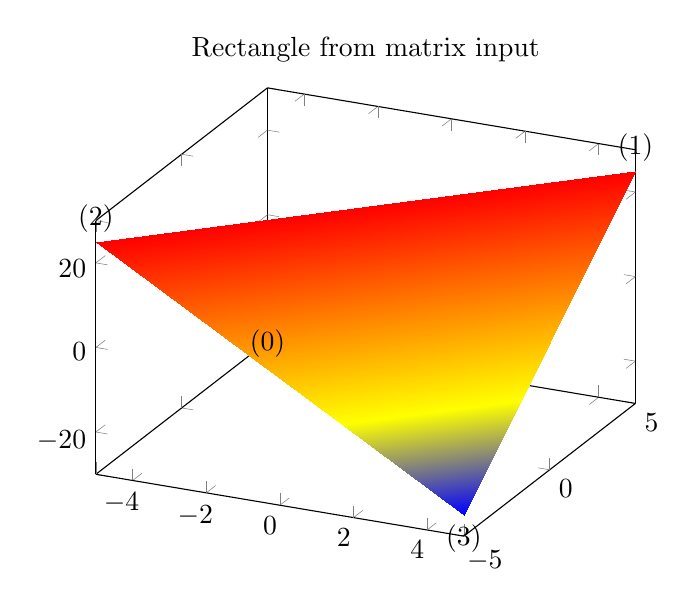
\begin{tikzpicture}
\begin{axis}[
    nodes near coords={(\coordindex)},
    title=Rectangle from matrix input,
]
    % note that surf implies 'patch type=rectangle'
    \addplot3 [
        surf,
        shader=interp,
        samples=2,
        patch type=rectangle,
    ] {x*y};
\end{axis}
\end{tikzpicture}
\end{codeexample}

\begin{codeexample}[]
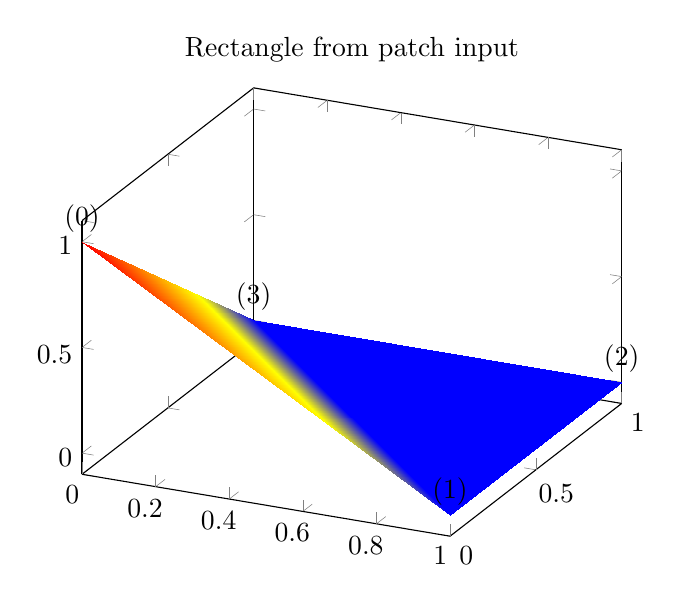
\begin{tikzpicture}
\begin{axis}[
    nodes near coords={(\coordindex)},
    title=Rectangle from patch input,
]
    \addplot3 [
        patch,
        shader=interp,
        patch type=rectangle,
    ] coordinates {
        (0,0,1) (1,0,0) (1,1,0) (0,1,0)
    };
\end{axis}
\end{tikzpicture}
\end{codeexample}
%
\noindent 如第~\pageref{key:patch:type} 页所述，|rectangle| 的 |shader=interp|
实现使用两个三角形并对其线性插值。上面两个例子的差异源于 $z$ 缓冲方式：矩阵输入
在线性时间内重排矩阵，而第二个例子会对完整矩形排序。在本例中，这导致不同的
角点顺序。

选项 \declareandlabel{bilinear} 在输入格式与描边路径上与 |rectangle| 基本相同，
但它为 |shader=interp| 使用正确的双线性着色。此外，几何也按双线性插值，而不仅是
两个三角形。上面两个例子现在变为
%
\begin{codeexample}[]
\begin{tikzpicture}
\begin{axis}[
    nodes near coords={(\coordindex)},
    title=Bilinear from $2\times 2$ matrix input,
]
    % note that surf implies 'patch type=rectangle'
    \addplot3 [
        surf,
        shader=interp,
        samples=2,
        patch type=bilinear,
    ] {x*y};
\end{axis}
\end{tikzpicture}
\end{codeexample}

\begin{codeexample}[]
\begin{tikzpicture}
\begin{axis}[
    nodes near coords={(\coordindex)},
    title=Bilinear from $4$--point patch input,
]
    \addplot3 [
        patch,
        shader=interp,
        patch type=bilinear,
    ] coordinates {
        (0,0,1) (1,0,0) (1,1,0) (0,1,0)
    };
\end{axis}
\end{tikzpicture}
\end{codeexample}
%
\noindent 若希望改善单个面片的形状与颜色插值质量，请使用 |patch type=bilinear|。
与更简单的 |patch type=rectangle| 相比，它可能导致输出文档更大。

选项 \declaretext{triangle} 期望一系列线性三角形，每个用 $n=3$ 个顶点编码：
%
\begin{codeexample}[]
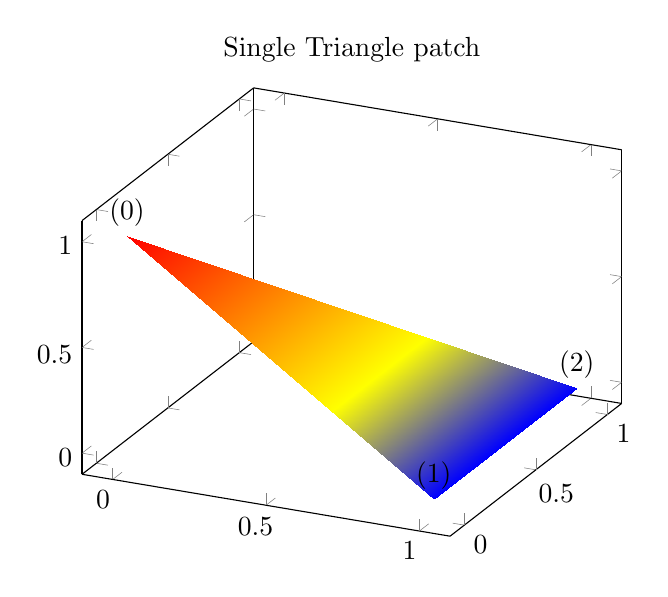
\begin{tikzpicture}
\begin{axis}[
    enlargelimits,
    nodes near coords={(\coordindex)},
    title=Single Triangle patch,
]
    \addplot3 [
        patch,
        shader=interp,
    ] coordinates {
        (0,0,1)
        (1,0,0)
        (1,1,0)
    };
\end{axis}
\end{tikzpicture}
\end{codeexample}

选项 \declareandlabel{triangle quadr} 期望一系列等参二次三角形，每个由 $n=6$ 个
顶点定义：
%
\begin{codeexample}[]
\begin{tikzpicture}
\begin{axis}[
    nodes near coords={(\coordindex)},
    title=Quadratic Triangle,
]
    \addplot [
        patch,
        patch type=triangle quadr,
        shader=interp,
        point meta=explicit,
    ] coordinates {
        (0,0) [1] (5,4) [2] (0,7) [3]
        (2,3) [1] (3,6) [2] (-1,4)  [3]
    };
\end{axis}
\end{tikzpicture}
\end{codeexample}

\begin{codeexample}[]
\begin{tikzpicture}
\begin{axis}[
    nodes near coords={(\coordindex)},
    title=Quadratic Triangle,
]
    \addplot3 [
        patch,
        patch type=triangle quadr,
        shader=interp,
    ] coordinates {
        (0,0,1) (5,4,0) (0,7,0)
        (2,3,0) (3,6,0) (-1,4,0)
    };
\end{axis}
\end{tikzpicture}
\end{codeexample}

\noindent 这里，边具有正确的二次形状。然而，颜色插值只是\emph{双线性}的；它使用
角点的颜色值而忽略其余部分（考虑使用 |patch refines| 改善颜色插值）。对于三维，
\PGFPlots{} 检查角点深度以决定前景/背景。对于二维，强烈扭曲的单元可能以意外方式
相互折叠。

选项 \declareandlabel{biquadratic} 期望一系列等参双线性四边形，每个由 $n=9$ 个
顶点定义。其主要用途是得到边界平滑的“矩形”：
%
\begin{codeexample}[]
\begin{tikzpicture}
\begin{axis}[
    nodes near coords={(\coordindex)},
    title=Single Biquadratic Quadrilateral,
]
    \addplot [
        patch,
        patch type=biquadratic,
        shader=interp,
        point meta=explicit,
    ] coordinates {
        (0,0) [1] (6,1) [2] (5,5) [3] (-1,5) [4]
        (3,1) [1] (6,3) [2] (2,6) [3] (0,3) [4]
        (3,3.75) [4]
    };
\end{axis}
\end{tikzpicture}
\end{codeexample}

\begin{codeexample}[]
\begin{tikzpicture}
\begin{axis}[
    nodes near coords={(\coordindex)},
    title=Single Biquadratic Quadrilateral,
]
    \addplot3 [
        patch,
        patch type=biquadratic,
        shader=interp,
    ] coordinates {
        (0,0,1) (6,1,0) (5,5,0) (-1,5,0)
        (3,1,0) (6,3,0) (2,6,0) (0,3,0)
        (3,3.75,0)
    };
\end{axis}
\end{tikzpicture}
\end{codeexample}
%
\noindent 与 |triangle quadr| 类似，边具有正确的二次形状——但颜色插值只是
\emph{双线性}的；它使用角点的颜色值而忽略其余部分。同样，请确保网格宽度足够小，
以改善颜色插值质量（另见 |patch refines|）。

注意，若 $(x,y)$ 的函数在 $y=\text{const}$ 时关于 $x$ 是二次的，且在
$x=\text{const}$ 时关于 $y$ 也是二次的，则它是双二次的（注意这不是“当且仅当”）。
例如，$f(x,y) = x^2-y^2$ 是双二次的。因此，我们只需一个双二次面片即可表示 $f$
的曲面图——只是颜色插值是双线性的。我们使用
|\addplot table[z expr=|\meta{expression}|]| 来实现：
%
\pgfplotsexpensiveexample
\begin{codeexample}[]
\begin{tikzpicture}
\begin{axis}
    \addplot3 [patch,patch refines=3,
        shader=faceted interp,
        patch type=biquadratic,
    ] table [z expr=x^2-y^2] {
        x  y
        -2 -2
        2  -2
        2  2
        -2 2
        0  -2
        2  0
        0  2
        -2 0
        0  0
    };
    \end{axis}
\end{tikzpicture}
\end{codeexample}
%
\noindent 我们看到，形状边界用 |biquadratic| 面片精确重建。此外，|patch refines|
改善了（一阶）颜色插值。|patch refines| 的细节见
第~\ref{sec:lib:patchplots:refinement} 节，叠加网格线的细节与限制见
第~\ref{sec:lib:patchplots:grids} 节。

注意，|biquadratic| 可以轻松与 |patch type sampling| 组合，以便对具有平滑边界的
任意 |surf|ace 曲面图采样。

类型为 |biquadratic| 且 |shader=interp| 的面片，其包围盒由输入顶点确定。由于面片
阶数较高，面片的某些部分可能位于该包围盒之外。这对所有高级面片类型都成立。
\index{Patch plots!Bounding Box}

选项 \declareandlabel{bicubic} 与 |biquadratic| 类似：它允许定义边界由四个三次
多项式构成的二维面片。因此，它允许非常平滑的边界——尤其是因为查看器在每个缩放
级别都会重新构建这些边界。|bicubic| 面片由 $16$ 个点构成，这些点排列成 $4\times4$
矩阵。每连续 $16$ 个点构成一个 |bicubic| 面片。第 $17$ 个点开始下一个
|bicubic| 面片（与其他任何 |patch type| 相同）。
%
\begin{codeexample}[]
\begin{tikzpicture}
\begin{axis}[
    nodes near coords={(\coordindex)},
    title=Single Bicubic Quadrilateral,
]
    \addplot3 [
        patch,
        patch type=bicubic,
        shader=interp,
    ] coordinates {
        (0,0,1) (1,0,0) (2,0,0) (3,0,0)
        (0,1,0) (1,1,0) (2,1,0) (3,1,0)
        (0,2,0) (1,2,0) (2,2,0) (3,2,0)
        (0,3,0) (1,3,0) (2,3,0) (3,3,0)
    };
\end{axis}
\end{tikzpicture}
\end{codeexample}
%
与 |biquadratic| 一样，|bicubic| 的颜色插值（只是）双线性的，尽管几何是高阶的。
颜色插值使用每个面片四个角点处确定的 |point meta| 值；着色器会忽略 |point meta|
的所有其他值（尽管这些值仍用于计算 |point meta min| 与 |point meta max|）。
%
\begin{codeexample}[]
\begin{tikzpicture}
\begin{axis}[title=Two Bicubic Patches]
    \addplot3 [patch,patch type=bicubic,
        shader=interp,point meta=explicit,
    ] coordinates {
        (0,0,1)[1] (1,0,0)[0] (2,0,0)[0] (3,0,0)[0]
        (0,1,0)[0] (1,1,0)[0] (2,1,0)[0] (3,1,0)[0]
        (0,2,0)[0] (1,2,0)[0] (2,2,0)[0] (3,2,0)[0]
        (0,3,0)[0] (1,3,0)[0] (2,3,0)[0] (3,3,0)[0]

        (3,0,0)[0] (4,0,0)[0] (5,0,0)[0] (6,0,0)[0.7]
        (3,1,0)[0] (4,1,.5)[1](5,1,0)[0] (6,1,0)[0]
        (3,2,0)[0] (4,2,0)[0] (5,2,0)[0] (6,2,0)[0]
        (3,3,0)[0] (4,3,0)[0] (5,3,0)[0] (6,3,0)[0.1]
    };
\end{axis}
\end{tikzpicture}
\end{codeexample}
%
上例使用两个 |bicubic| 类型的面片。注意，颜色数据（|point meta|）是显式提供的
——但其值仅在角点处使用（点 |(4,1,.5)| 后的 |[1]| 值被忽略）。|bicubic| 面片的
颜色插值仅使用面片角点处的颜色数据。其余颜色数据值被忽略。注意，若保留默认
（即 |point meta=f(x)| 而非 |point meta=explicit|），第二个面片将是蓝色。这是因为
第二个面片的四个角点顶点决定了颜色着色——而它们的 $z$ 值为~$0$。

注意，|bicubic| 可以轻松与 |patch type sampling| 组合，以便对具有平滑边界的任意
|surf|ace 曲面图采样。

如 |biquadratic| 所述，类型为 |bicubic| 且 |shader=interp| 的面片，其包围盒可能
比实际绘制区域略小（因为包围盒由输入点计算）。

选项 \declareandlabel{coons} 期望一个或多个 Coons 面片，每个由 $n=12$ 个点构成。
Coons 面片由四条三次贝塞尔曲线围成，端点彼此相连——这 $n$ 个点以特定顺序提供
这些曲线所需的控制点，顺序如下例所示：
%
\begin{codeexample}[]
\begin{tikzpicture}
    \begin{axis}[
        nodes near coords={(\coordindex)},
        width=12cm,
        title=A Coons Patch,
    ]
        \addplot [mark=*,patch,patch type=coons,
            shader=interp,point meta=explicit,
        ] coordinates {
            (0,0)      [0] % first corner
            (1,-1)     [0] % Bezier control point between (0) and (3)
            (4,0.7)    [0] % Bezier control point between (0) and (3)
            %
            (3,2)      [1] % second corner
            (4,3.5)    [1] % Bezier control point between (3) and (6)
            (7,2)      [1] % Bezier control point between (3) and (6)
            %
            (7,1)      [2] % third corner
            (6,0.6)    [2] % Bezier control point between (6) and (9)
            (4.5,-0.5) [2] % Bezier control point between (6) and (9)
            %
            (5,-2)     [3] % fourth corner
            (4,-2.5)   [3] % Bezier control point between (9) and (0)
            (-1,-2)    [3] % Bezier control point between (9) and (0)
        };
    \end{axis}
\end{tikzpicture}
\end{codeexample}
%
\noindent 这四条三次贝塞尔曲线\emph{等价于} \pgfname{} 的 \texttt{curveto}
路径，即形如
\parg{corner~1}| .. controls |\parg{control~point~A}| and |\parg{control~point~B}| .. |\parg{corner 2}
的序列。插值着色是双线性的。更准确地说，先在单位正方形 $[0,1]^2$ 中初始化一个
双线性着色，然后将其映射到 Coons 面片，使角点匹配。颜色插值仅使用四个角点的
颜色数据；中间控制点的颜色值在着色中被忽略（不过其值仍会纳入颜色数据的上下限）。
与有限元面片不同，Coons 面片本质上是二维的。虽然仍可使用三维坐标，但
\PGFPlots{} 会按你提供的方式绘制着色，而不检查深度信息（它对其他 |patch type|
会检查）。换句话说：根据当前 |view| 视角，着色可能以意外方式自身折叠。

即使在二维中，Coons 面片也可能自身折叠。为判断哪部分是前景、哪部分是背景，
采用如下规则：四个角点 $(0)$、$(3)$、$(6)$、$(9)$ 分别对应单位正方形点
$(u,v)=(0,0)$、$(0,1)$、$(1,1)$ 与 $(1,0)$。角点 $(3)$ 与 $(6)$ 之间的边
（即 $v=1$ 的边）是前景，角点 $(1)$ 与 $(9)$ 之间的边是背景。因此，较大的 $v$
值绘制在较小的 $v$ 值之上。若 $v$ 为常数，则较大的 $u$ 值绘制在较小的 $u$ 值
之上。因此，重排面片顶点（选择不同的第一个顶点和/或反转顺序）可得到不同的
前景/背景配置。\footnote{在内部，\PGFPlots{} 使用此类机制将高阶等参面片类型
映射到 Coons 面片，并按角点深度信息排序。}

注意，|patch type=coons| 不可用 |patch type sampling|，因为控制点并非同一函数的
点求值。

选项 \declareandlabel{tensor bezier} 与 |patch type=coons| 类似：它允许定义贝塞尔
面片。但它提供更多自由度：它有 $16$ 个控制点，而不是 |coons| 面片的 $12$ 个。
额外四个控制点位于每个面片的中心。该 |patch type| 生成类型为~$7$ 的
\texttt{.pdf} 着色（而 |coons| 面片是类型~$6$ 的着色）。它是为完整性而添加的，
尽管尚未经过充分测试。细节请参考 \texttt{.pdf} 格式规范。\footnote{若有人愿意
测试并记录它，欢迎给我发邮件！}
选项 |tensor bezier| 实际上与 |patch type=bicubic| \emph{相同}——只是
|bicubic| 自动尊重视图深度（前景/背景），并且通过函数求值而非控制点给出。

注意，|patch type=tensor bezier| 不可用 |patch type sampling|，因为控制点并非
同一函数的点求值。

选项 \declareandlabel{polygon} 期望具有固定顶点数的多边形。该 |patch type| 要求
将顶点数作为参数：

\begin{pgfplotskey}{vertex count=\meta{count}}
    用于 |patch type=polygon| 的顶点数。该数可以任意。所有输入面片都应有这么多
    顶点——但允许一个面片多次使用同一顶点。这意味着 |patch type=polygon| 接受
    不同顶点数的多边形，但你需要进行某种“手动填充”。

    该参数（目前）是必需的。
\end{pgfplotskey}

使用 |patch type=polygon| 的 |patch| 图只是按出现顺序连接 $n$=|vertex count| 个
顶点，并闭合所得路径：
%
\begin{codeexample}[]
\begin{tikzpicture}
\begin{axis}[view/h=120,xlabel=$x$,ylabel=$y$]
    \addplot3 [
        opacity=0.5,
        table/row sep=\\,
        patch,
        patch type=polygon,
        vertex count=5,
        patch table with point meta={
            % pt1 pt2 pt3 pt4 pt5 cdata
            0 1 7 2 2 0\\
            1 6 5 5 5 1\\
            1 5 4 2 7 2\\
            2 4 3 3 3 3\\
        },
    ] table {
        x y z\\
        0 2 0\\%0
        2 2 0\\%1
        0 1 3\\%2
        0 0 3\\%3
        1 0 3\\%4
        2 0 2\\%5
        2 0 0\\%6
        1 1 2\\%7
    };
    % replicate the vertex list to show \coordindex:
    \addplot3 [only marks,
        nodes near coords=\coordindex,
    ] table [row sep=\\] {
        0 2 0\\ 2 2 0\\ 0 1 3\\ 0 0 3\\
        1 0 3\\ 2 0 2\\ 2 0 0\\ 1 1 2\\
    };
\end{axis}
\end{tikzpicture}
\end{codeexample}
%
\noindent 上面的例子通过连通性表（|patch table with point meta|）与顶点列表
（图的普通输入坐标）定义 |patch|：有~$8$ 个顶点与~$4$ 个多边形。注意，其中
~$2$ 个多边形是三角形，一个有 $4$ 个角，只有一个真正拥有全部~$5$ 个分配的角。
这种效果可以通过重复某个角实现。本例中的连通性表为每个多边形定义唯一颜色：
第一个面片为 $0$，第二个为 $1$，第三个为 $2$，最后一个为 $3$。这些数字映射到
当前 |colormap|。

|patch type=polygon| \emph{既不}支持三角剖分，\emph{也不}支持着色，\emph{也不}
支持细化。输入点的出现顺序即为所得路径中 line-to 操作生成的顺序。


\subsection{自动面片细化与三角剖分}
\label{sec:lib:patchplots:refinement}

\PGFPlots{} 对其大多数 |patch type| 支持自动面片细化。面片细化主要有两个目的：
提高 |z buffer=sort| 的质量，和/或改善高阶面片的颜色插值。

\begin{pgfplotskey}{patch refines=\marg{levels} (initially 0)}
    该键控制面片细化。初始选项 |patch refines=0| 禁用细化，按输入文件中找到的
    单元原样可视化。

    正的 \meta{levels} 启用（递归）面片细化：每个面片单独细化。

    下面的例子以边上的 |triangle quadr| 形状函数说明 |patch refines| 特性。
    注意，由于 \PGFPlots{} 仅使用基于角点 $(0)$、$(1)$ 与 $(2)$ 的一阶着色，
    |patch refines=0| 指定的形状函数颜色为常量。更大的 \meta{levels} 以递增
    质量近似面片：
    %
\begin{codeexample}[]
\foreach \level in {0,1,2} {%
    \begin{tikzpicture}
        \begin{axis}[
            nodes near coords={(\coordindex)},
            footnotesize,
            title={patch refines = \level},
        ]
            \addplot3 [patch,patch type=triangle quadr,
                shader=faceted interp,patch refines=\level,
            ] coordinates {
                (0,0,0) (5,4,0) (0,7,0)
                (2,3,0) (3,6,1) (-1,4,0)
            };
        \end{axis}
    \end{tikzpicture}
}
\end{codeexample}
    %
    \noindent 本例中，面片细化效果显著，因为它只是一个位移巨大的单元。对实际
    例子，你大概不需要太多细化级别。

    细化后的面片精确复现几何形状。此外，它们改善颜色插值。注意，其目的只是
    可视化，因此允许悬挂节点（对大多数 |patch type|，|patch refines| 会生成
    悬挂节点）。

    除 |patch type=coons|、|tensor bezier|、|bicubic|（将来可能支持）与
    |polygon| 外，所有受支持面片都实现了面片细化。
\end{pgfplotskey}

\begin{pgfplotskey}{patch to triangles=\mchoice{true,false} (initially false)}
    有时，输入是复杂的 |patch type|，希望将其可视化为 |triangle| 网格。
    \PGFPlots{} 支持面片自动三角剖分。三角剖分即用一个或多个三角形替换每个输入
    面片。三角剖分可与 |patch refines| 组合，此时先应用 |patch refines|，再对
    所得细化面片进行三角剖分。
    %
\begin{codeexample}[]
\foreach \level in {0,1,2} {%
    \begin{tikzpicture}
        \begin{axis}[
            nodes near coords={(\coordindex)},
            footnotesize,
            title={Triangulation + \level\ refines},
        ]
            \addplot3 [patch,patch type=biquadratic,shader=faceted interp,
                patch to triangles,patch refines=\level,
            ] coordinates {
                (0,0,0) (6,1,0) (5,5,0) (-1,5,0)
                (3,1,0) (6,3,0) (2,6,0) (0,3,0)
                (3,3.75,1)
            };
        \end{axis}
    \end{tikzpicture}%
}
\end{codeexample}

    对于 |quadratic spline| 等一维 |patch type|，|patch to triangles| 会改用
    |patch type=line| 近似，而不是 |triangle|。

    除 |patch type=coons|、|tensor bezier| 与 |polygon| 外，所有受支持面片都实现了
    |patch to triangles| 特性。
\end{pgfplotskey}


\subsection{平面着色与高阶面片的特性}
\label{sec:lib:patchplots:flat}

|patchplots| 库针对插值着色进行了优化，即针对 |shader=interp|：它允许填充区域
自身折叠或超出面片边界。

\PGFPlots{} 也通过简单地描边和/或填充面片边界来支持 |shader=flat| 与
|shader=faceted|。自然地，这种方法只有在被包围的面片边界与填充区域基本一致时
才有效！仅当\emph{网格宽度足够小}、面片不会自身折叠时，才考虑使用
|shader=flat| 或 |shader=faceted|。

下面的例子说明效果：左侧粗糙的单一单元自身折叠，产生奇怪的填充图案。细化网格
可减弱该效果。
%
\begin{codeexample}[]
\foreach \level in {0,1,2} {%
    \begin{tikzpicture}
        \begin{axis}[
            footnotesize,
            title={Faceted + \level\ refines},
        ]
            \addplot3 [patch,patch type=biquadratic,shader=faceted,
                patch refines=\level,
            ] coordinates {
                (0,0,1) (6,1,0) (5,5,0) (-1,5,0)
                (3,1,0) (6,3,0) (2,6,0) (0,3,0)
                (3,3.75,0)
            };
        \end{axis}
    \end{tikzpicture}
}
\end{codeexample}


\subsection{绘制网格}
\label{sec:lib:patchplots:grids}

|patchplots| 库以与二维/三维 |mesh| 和 |surf| 图相同的方式支持网格（|mesh|）
可视化。这包括四种不同方法：第一种是 |shader=faceted|，它对填充使用常量颜色，
对描边路径使用 |faceted color|（我们已在第~\ref{sec:lib:patchplots:flat} 节看到）。
第二种方法是使用 |shader=faceted interp|，它使用插值着色填充，并在每个插值单元
之上发出描边路径。第三种方法是发出两条 |\addplot| 命令：一条带填充的 |patch| 图，
一条带 |patch,mesh| 样式，后者仅在前一个图之上绘制（彩色）网格线。三种方法如下
所示。
%
\begin{codeexample}[]
\begin{tikzpicture}
\begin{axis}[
    title={Grids with shader=faceted},
]
    \addplot3 [patch,patch type=biquadratic,
        shader=faceted,patch refines=3,
    ] coordinates {
        (0,0,1) (6,1,1.6) (5,5,1.3) (-1,5,0)
        (3,1,0) (6,3,0.4) (2,6,1.1) (0,3,0.9)
        (3,3.75,0.5)
    };
\end{axis}
\end{tikzpicture}
\end{codeexample}
%
\noindent 如第~\ref{sec:lib:patchplots:flat} 节所述，若网格宽度足够小（使单个
面片不重叠、填充区域位于面片边界内），|shader=faceted| 方法效果良好。
%
\begin{codeexample}[]
\begin{tikzpicture}
\begin{axis}[
    title={Grids with shader=faceted interp},
]
    \addplot3 [patch,patch type=biquadratic,
        shader=faceted interp,patch refines=3]
    coordinates {
        (0,0,1) (6,1,1.6) (5,5,1.3) (-1,5,0)
        (3,1,0) (6,3,0.4) (2,6,1.1) (0,3,0.9)
        (3,3.75,0.5)
    };
\end{axis}
\end{tikzpicture}
\end{codeexample}
%
\noindent 这里，网格线被定义为面片边界，因此对于粗糙面片，偶尔会出现网格线穿过
填充区域的情况。若遇到问题，请考虑使用 |patch refines| 键。|shader=faceted interp| 支持 |z buffer|——代价是为\emph{每个}面片单元生成一个着色（描边路径在面片
单元着色后立即绘制）。这在显示时可能相当昂贵\footnote{我非常希望听到任何有根据的
改进思路。若你有想法——请告诉我！}，并可能导致巨大的 PDF 文件。然而，
|shader=faceted interp| 同时提供平滑着色与按正确顺序绘制的良好网格线。
%
\begin{codeexample}[]
\begin{tikzpicture}
\begin{axis}[
    title={Mesh on top of patches (i): obscured},
]
    \addplot3 [patch,patch type=biquadratic,
        shader=interp,patch refines=3,
    ] coordinates {
        (0,0,1) (6,1,1.6) (5,5,1.3) (-1,5,0)
        (3,1,0) (6,3,0.4) (2,6,1.1) (0,3,0.9)
        (3,3.75,0.5)
    };
    \addplot3 [patch,patch type=biquadratic,
        mesh,black,patch refines=3,
    ] coordinates {
        (0,0,1) (6,1,1.6) (5,5,1.3) (-1,5,0)
        (3,1,0) (6,3,0.4) (2,6,1.1) (0,3,0.9)
        (3,3.75,0.5)
    };
\end{axis}
\end{tikzpicture}
\end{codeexample}

\begin{codeexample}[]
\begin{tikzpicture}
\begin{axis}[
    title={Mesh on top of patches (ii): unobscured\\
      \tiny Geometry provided by Prof. Chernov, Bonn},
    title style={align=center},
    view={156}{28},
]
    \addplot3 [patch,patch type=bilinear,
        shader=interp,
        patch table=plotdata/patchexample_conn.dat,
    ] file {plotdata/patchexample_verts.dat};

    \addplot3 [patch,patch type=bilinear,
        mesh,black,
        patch table=plotdata/patchexample_conn.dat,
    ] file {plotdata/patchexample_verts.dat};
\end{axis}
\end{tikzpicture}
\end{codeexample}
%
\noindent 单独绘制网格的方法通过两条 |\addplot| 语句实现：第一条像以前一样使用
|patch|，第二条使用 |patch,mesh|。这配置 \PGFPlots{} 仅可视化网格。请确保在
|patch| 之后提供 |mesh|，因为后者会激活填充的 |surf| 可视化。面片之上叠加网格
的方法意味着网格线简单地绘制在任何先前绘图操作之上。因此，深度信息丢失（如上面
第一个例子所示）。在特殊情况下，将网格线叠加在曲面之上可行（见下图）。一种始终
可行的方法是将网格放在固定 $z$ 位置，如下例所示：
%
\begin{codeexample}[]
\begin{tikzpicture}
\begin{axis}[
    title={Separate Grids (iii)},
]
    \addplot3 [patch,patch type=biquadratic,
        shader=interp,patch refines=3,
    ] coordinates {
        (0,0,1) (6,1,1.6) (5,5,1.3) (-1,5,0)
        (3,1,0) (6,3,0.4) (2,6,1.1) (0,3,0.9)
        (3,3.75,0.5)
    };
    \addplot3 [patch,patch type=biquadratic,
        mesh,black,
        z filter/.code={\def\pgfmathresult{1.8}},
        patch refines=3,
    ] coordinates {
        (0,0,1) (6,1,1.6) (5,5,1.3) (-1,5,0)
        (3,1,0) (6,3,0.4) (2,6,1.1) (0,3,0.9)
        (3,3.75,0.5)
    };
\end{axis}
\end{tikzpicture}
\end{codeexample}
%
\noindent 这里，第一条 |\addplot3| 命令与上面相同，只是使用 |shader=interp|。
第二条复现相同几何，但使用 |z filter| 固定 $z$ 坐标（本例为 $z=1.8$）。这有效地
覆盖了所有 $z$ 坐标。

因此，网格线既可以通过 |shader=faceted| 的平面填充色绘制（高效），也可以通过
|shader=faceted interp| 的插值填充色绘制（低效，见上），或在特殊应用中使用单独的
|patch,mesh| 图绘制在面片之上（高效）。无论如何，网格可视化会考虑
|faceted color|，它可依赖 |mapped color|。

\end{pgfplotslibrary}
}
